\begin{tikzpicture}[node distance=3.4cm and 2.3cm]

    % ----------------------------------------------------------
    % (1) mean-value vector  --- one row per intervention
    % ----------------------------------------------------------
    \node[matrixbox] (meanvec) {
      \begin{tikzpicture}[scale=0.65,baseline]
        % 5×1 column vector grid
        \foreach \i in {0,...,5}{
          \draw[very thin,gray!65] (0,\i) -- (1,\i);
        }
        \draw[very thin,gray!65] (0,0) -- (0,5);
        \draw[very thin,gray!65] (1,0) -- (1,5);
      \end{tikzpicture}
    };
    \node[below=4pt of meanvec,align=center]
      {\scriptsize Mean size / risk\\[-1pt]\scriptsize per intervention};
    
    % ----------------------------------------------------------
    % (2) five membership vectors (via fuzzy c-means)
    % ----------------------------------------------------------
    \foreach \name/\x/\col in {small/0/s0, midsmall/1/s1, medium/2/s2, midlarge/3/s3, large/4/s4}{
      \node[fuzzymatrix=\col,right=of meanvec,xshift={(\x)*0.34cm-0.34cm}] (V\name){
        \begin{tikzpicture}[scale=0.65]
          \foreach \i in {0,...,5}{
            \draw[very thin,white] (0,\i) -- (1,\i);
          }
          \draw[very thin,white] (0,0) -- (0,5);
          \draw[very thin,white] (1,0) -- (1,5);
        \end{tikzpicture}
      };
    }
    \node[below=4pt of Vmedium,align=center]
      {\scriptsize 5 fuzzy membership vectors\\[-1pt]\scriptsize (one per cluster)};
    
    % ----------------------------------------------------------
    % (3) active-interventions vector for day \(t\) (blue-square style)
    % ----------------------------------------------------------
    \node[matrixbox,right=of Vlarge,xshift=1.1cm] (active) {
      \begin{tikzpicture}[scale=0.65,baseline]
        % 5×1 column vector grid
        \foreach \i in {0,...,5}{
          \draw[very thin,gray!65] (0,\i) -- (1,\i);
        }
        \draw[very thin,gray!65] (0,0) -- (0,5);
        \draw[very thin,gray!65] (1,0) -- (1,5);
        % blue shading for 1st, 3rd, and 5th cells
        \foreach \y in {0,2,4}{
          \fill[s0!28] (0,\y) rectangle ++(1,1);
        }
      \end{tikzpicture}
    };
    \node[below=5pt of active,align=center]
      {\scriptsize active interventions\\[-1pt]\scriptsize at day $t$};
    
    % ----------------------------------------------------------
    % (4) daily mass series
    % ----------------------------------------------------------
    \node[matrixbox,right=of active] (mass) {
      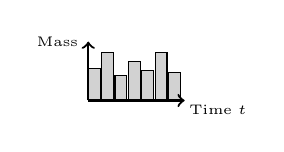
\begin{tikzpicture}[scale=0.34,baseline]
        \foreach \t/\h in {0/1.2,1/1.8,2/0.95,3/1.45,4/1.13,5/1.8,6/1.05}{
          \draw[fill=gray!35] (\t*0.50,0) rectangle ++(0.44,\h);
        }
        \draw[->,thick] (0,0) -- (3.6,0) node[below right=-2pt] {\tiny Time $t$};
        \draw[->,thick] (0,0) -- (0,2.2) node[left] {\tiny Mass};
      \end{tikzpicture}
    };
    \node[below=4pt of mass] {\scriptsize daily mass series $M(t)$};
    
    % ----------------------------------------------------------
    % (5) entropy scores
    % ----------------------------------------------------------
    \node[scalarbox,right=of mass] (entropy)
      {\Large$-\displaystyle\frac{H\!\bigl(M_{\text{norm}}\bigr)}{H_{\text{unif}}}$};
    \node[below=4pt of entropy,align=center]
      {\scriptsize 5 normalised entropy scores\\[-1pt]\scriptsize (one for each fuzzy cluster)};
    
    % ----------------------------------------------------------
    % arrows
    % ----------------------------------------------------------
    \draw[arrow] (meanvec.east) -- ++(1.0,0) -- (Vsmall.west)
      node[process,above,yshift=12pt,pos=0]{fuzzy\,c-means\\clustering};
    
    \draw[arrow] (Vlarge.east) -- ++(0.9,0) -- (active.west)
      node[process,above,yshift=12pt,pos=0.35]{\textbf{for each of the 5}\\membership vectors select\\active interventions\\for each day};
    
    \draw[arrow] (active.east) -- (mass.west)
      node[process,above,yshift=12pt,pos=0.5]{aggregate\\per day};
    
    \draw[arrow] (mass.east) -- (entropy.west)
      node[process,above,yshift=12pt,pos=0.5]{normalise by\\total mass};
    
    \end{tikzpicture}